\documentclass{chi-ext}
% Please be sure that you have the dependencies (i.e., additional LaTeX packages) to compile this example.
% See http://personales.upv.es/luileito/chiext/

%% EXAMPLE BEGIN -- HOW TO OVERRIDE THE DEFAULT COPYRIGHT STRIP -- (July 22, 2013 - Paul Baumann)
\copyrightinfo{Permission to make digital or hard copies of all or part of this work for personal or classroom use is granted without fee provided that copies are not made or distributed for profit or commercial advantage and that copies bear this notice and the full citation on the first page. Copyrights for components of this work owned by others than ACM must be honored. Abstracting with credit is permitted. To copy otherwise, or republish, to post on servers or to redistribute to lists, requires prior specific permission and/or a fee. Request permissions from permissions@acm.org. \\
{\emph{ISS '17}}, October 17--20, 2017, Brighton, United Kingdom. \\
Copyright \copyright~2017 ACM ISBN 978-1-4503-4691-7/17/10. \\
10.1145/3132272.3135074}
%% EXAMPLE END -- HOW TO OVERRIDE THE DEFAULT COPYRIGHT STRIP -- (July 22, 2013 - Paul Baumann)

% \CopyrightYear{2017}
% \setcopyright{rightsretained}
% \conferenceinfo{ISS '17}{October 17--20, 2017, Brighton, United Kingdom}\isbn{978-1-4503-4691-7/17/10}
% \doi{https://doi.org/10.1145/3132272.3135074}



\title{Gesture Typing on Virtual Tabletop: Effect of Input Dimensions on Performance}

\numberofauthors{4}
% Notice how author names are alternately typesetted to appear ordered in 2-column format;
% i.e., the first 4 autors on the first column and the other 4 auhors on the second column.
% Actually, it's up to you to strictly adhere to this author notation.
\author{
  \alignauthor{
    \textbf{Antoine Loriette}\\
    \affaddr{Dept. Computing Science}\\
    \affaddr{University of Glasgow}\\
    \affaddr{Scotland, UK}\\
    \email{antoine.loriette@glasgow.ac.uk}
  }\alignauthor{
    \textbf{Sebastian Stein}\\
    \affaddr{Dept. Computing Science}\\
    \affaddr{University of Glasgow}\\
    \affaddr{Scotland, UK}\\
    \email{sebastian.stein@glasgow.ac.uk}
  }
  \vfil
  \alignauthor{
    \textbf{Roderick Murray-Smith}\\
    \affaddr{Dept. Computing Science}\\
    \affaddr{University of Glasgow}\\
    \affaddr{Scotland, UK}\\
    \email{rod@dcs.gla.ac.uk}
  }\alignauthor{
    \textbf{John Williamson}\\
    \affaddr{Dept. Computing Science}\\
    \affaddr{University of Glasgow}\\
    \affaddr{Scotland, UK}\\
    \email{jhw@dcs.gla.ac.uk}
  }
\vfil
}

% Paper metadata (use plain text, for PDF inclusion and later re-using, if desired)
\def\plaintitle{Gesture Typing on Virtual Surfaces: Effect of Input Dimensions on Performance}
\def\plainauthor{Name}
\def\plainkeywords{Indirect Interaction, Gesture Input, Gesture Keyboard, Mobile, Continuous Interaction, Tabletop, Text Input}
\def\plaingeneralterms{Documentation, Standardization}

\hypersetup{
  % Your metadata go here
  pdftitle={\plaintitle},
  pdfauthor={\plainauthor},
  pdfkeywords={\plainkeywords},
  pdfsubject={\plaingeneralterms},
  % Quick access to color overriding:
  %citecolor=black,
  %linkcolor=black,
  %menucolor=black,
  %urlcolor=black,
}

\usepackage{graphicx}   % for EPS use the graphics package instead
\usepackage{balance}    % useful for balancing the last columns
\usepackage{bibspacing} % save vertical space in references

\usepackage{subfigure}

% own command
\newcommand{\reffigure}[1]{Figure~\ref{#1}}
\newcommand{\reftable}[1]{Table~\ref{#1}}
\newcommand{\smit}[1]{{\small\textit{{#1}}}}
\newcommand{\cdt}[1]{{\small\uppercase{{#1}}}}
\newcommand{\wpm}{\cdt{wpm} }


\begin{document}

\maketitle

\begin{abstract}
The association of tabletop interaction with gesture typing presents interaction potential for situationally or physically impaired users. In this work, we use depth cameras to create touch surfaces on regular tabletops. We describe our prototype system and report on a supervised learning approach to fingertips touch classification. We follow with a gesture typing study that compares our system with a control tablet scenario and explore the influence of input size and aspect ratio of the virtual surface on the text input performance. We show that novice users perform with the same error rate at half the input rate with our system as compared to the control condition, that an input size between A5 and A4 present the best tradeoff between performance and user preference and that users' indirect tracking ability seems to be the overall performance limiting factor.
\end{abstract}

\keywords{\plainkeywords}
% \textcolor{red}{Optional section to be included in your final version.}

\category{H.5.m}{Information interfaces and presentation (e.g., HCI)}{Miscellaneous}.
%See \cite{ACMCCS}
% See: \url{http://www.acm.org/about/class/1998/}
% for help using the ACM Classification system.
% \textcolor{red}{Optional section to be included in your final version, but strongly encouraged.}


% =============================================================================
\section{Introduction}
% =============================================================================
The combination of indirect optically tracked input and potentially projected display (“virtual surfaces”) has several interesting properties. Virtual surfaces, as opposed to touch screens, are well suited to tackle the palm rejection problem and the occlusion problem, offer a choice of size, aspect ratio and texture of the input space, and allow interactions with dirty or wet hands.

Depth cameras~\cite{Harrison2011,Sridhar2017,Xiao2016} have usually been employed to create such surfaces, while other work have combined different sensor sources~\cite{Wen2016}. However, the touch classification, critical to the quality of the interaction remains challenging~\cite{Xiao2016} and is traditionally addressed by hand-tuning parameters and thresholding.

\marginpar{
\begin{figure}
    \begin{center}
        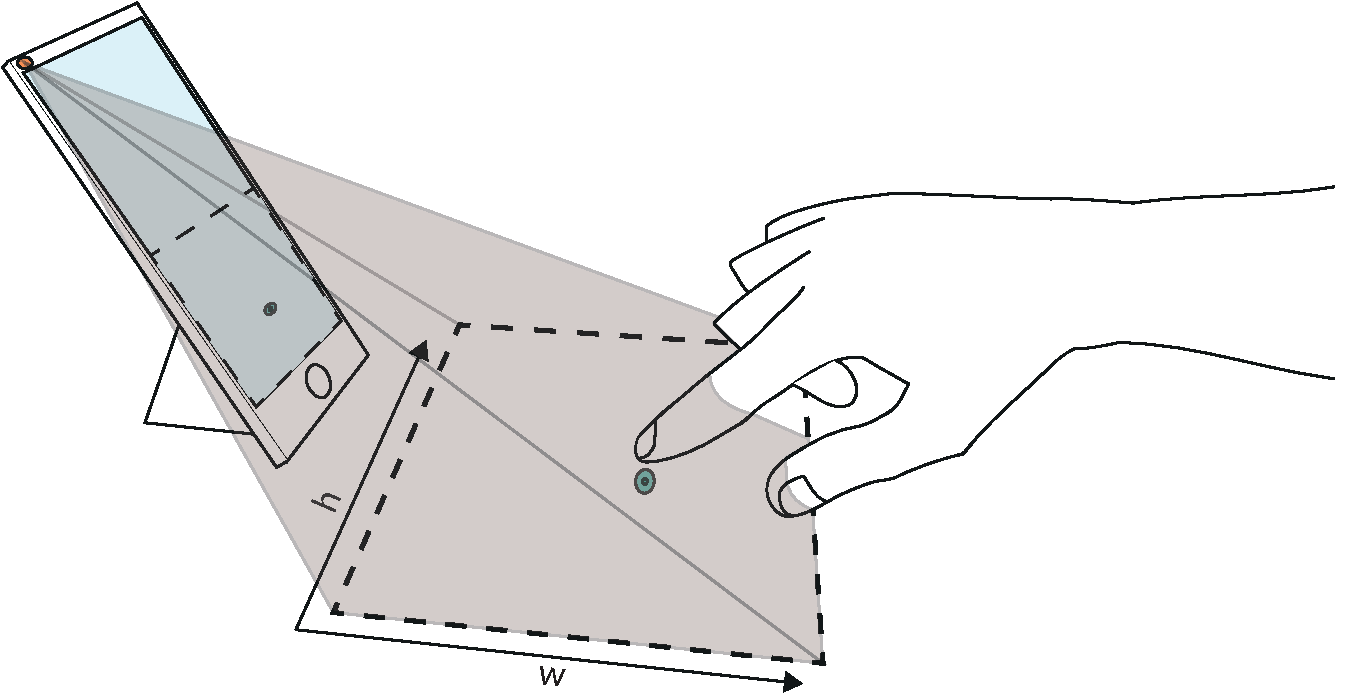
\includegraphics[width=\marginparwidth]{figures/banner.pdf}
        \caption{Potential interaction setup. A mobile device whose optical sensor creates an on-demand touch surface offers width and height as free parameters.}
        \label{fig:banner}
    \end{center}
\end{figure}
\begin{figure}
    \begin{center}
        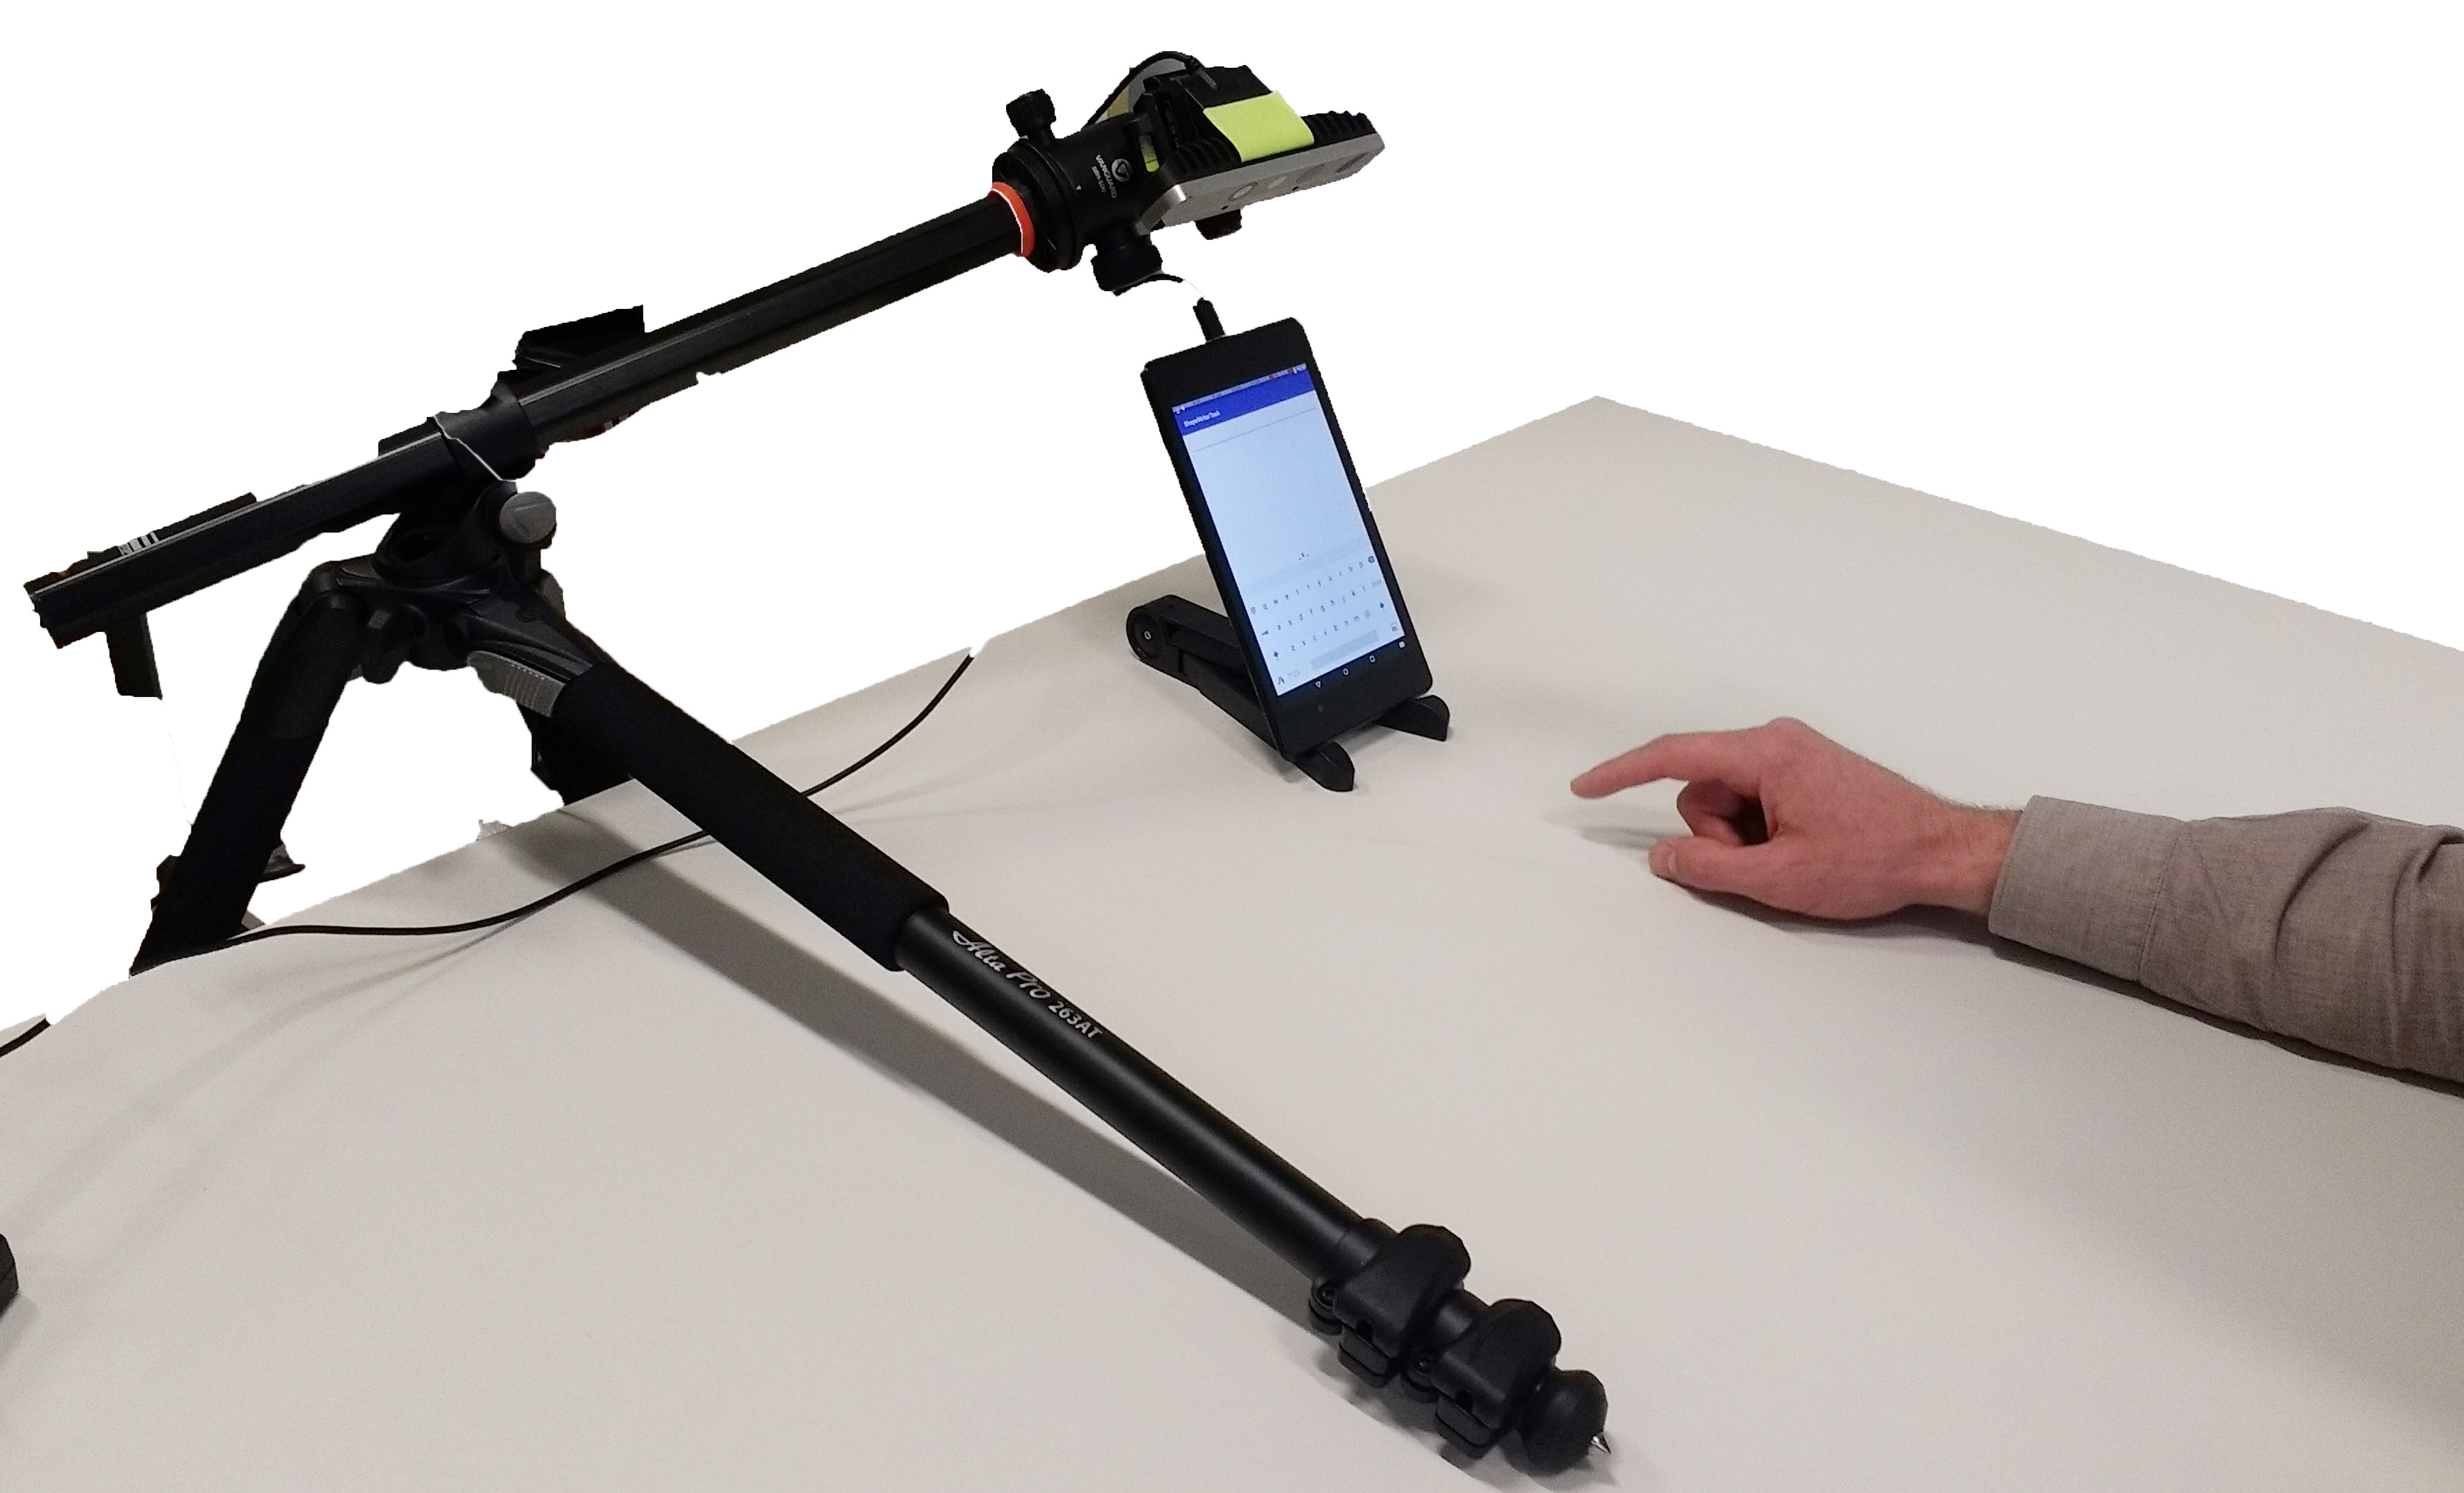
\includegraphics[width=\marginparwidth]{figures/system_insitu_0.jpg}
        \caption{Picture of the user study setup. A tablet device provides the audiovisual feedback while a depth camera mounted on a tripod creates a virtual touch input surface.}
        \label{fig:system_insitu_0}
    \end{center}
\end{figure}
}

In this context, the task of gesture typing~\cite{Kristensson2004} is an interesting research focus. Text-input is a major activity~\cite{McGregor2014} on mobile device taking up to 40\% of the user interaction time. The technique lends itself well to optical systems by limiting the requirement for repetitive target acquisition or touch classification. Yet, little is known about the impact of input size (one of the free parameters of virtual surfaces) on writing performance as other works focused on pointing~\cite{Casiez2008,Gilliot2014} or bimanual task~\cite{Schmidt2009}.

This work specifically focuses on two goals: to report on a supervised learning approach to the fingertip touch classification task and to study the influence of input space (size and aspect ratio) on gesture typing performance using virtual tabletops.

% =============================================================================
\section{System Overview}
% =============================================================================
The envisioned interaction scenario is shown in ~\autoref{fig:banner}. A camera overlooks the interaction surface and a computing device performs the hand and fingers tracking as well as the touch detection. The system map in an indirect manner the user's pointer from the virtual surface onto the device's screen. A 3-state button model is used with visual feedback indicating hover positions and continuous touches. Audio cues indicate whenever a new touch down event is detected.

\section{Touch Classification}
This task is well suited to a supervised learning approach provided a training dataset is available. One of the authors video-taped 6 minutes of interactions creating 3 distincts datasets for 3 different fingers (index, thumb and pinky) totalling 10800 frames. The datasets are balanced with regards to touching frames and hovering frames and include a minor portion of out-of-range frames. The classification features are chosen as 20-bins histograms of z-values of the detected fingertip pointcloud, in red on~\autoref{fig:pointcloud}, which provides some orientation and shape invariance.

This is fed to a binary neural network classifier: 20 inputs dimensions, 2 layers of 64 units with Relu activation and $0.5$ dropout, and a fully connected layer with sigmoid activation. We use the binary cross-entropy as loss function and rmsprop for the optimiser. We train the model over 50 epochs and cross-validate with 3 folds (different fingers are thus validated against each others). The generalisation over different fingers is satisfying as shown by the average performance of 0.96 AUC for the ROC, see~\autoref{fig:roc_auc}. The model used for the user study was trained over the full dataset over 75 epochs. As an improvment, it is worth noting the possibility to delegate the feature extraction step to a model capable of inferring features directly, such as a convolutional neural network.

% =============================================================================
\section{User Study}
% =============================================================================
We ran an experiment with two research goals in mind. First we wanted to evaluate the usability of our system, for this purpose we included a condition with an interaction directly on the tablet. Second, given the nature of the task and its inherent difficulty for novice users, we investigated the influence of the physical space on performance. Accot et al.~\cite{Accot2001} demonstrated a U-shaped curve in performance against input scale. Our independent variable were thus the control surface dimensions, which effectively change the control-display gain ($CD_{gain}$) defined as in \cite{Casiez2008} by the the ratio of the pointer velocity to device velocity.

\marginpar{
\begin{figure}
    \centering
    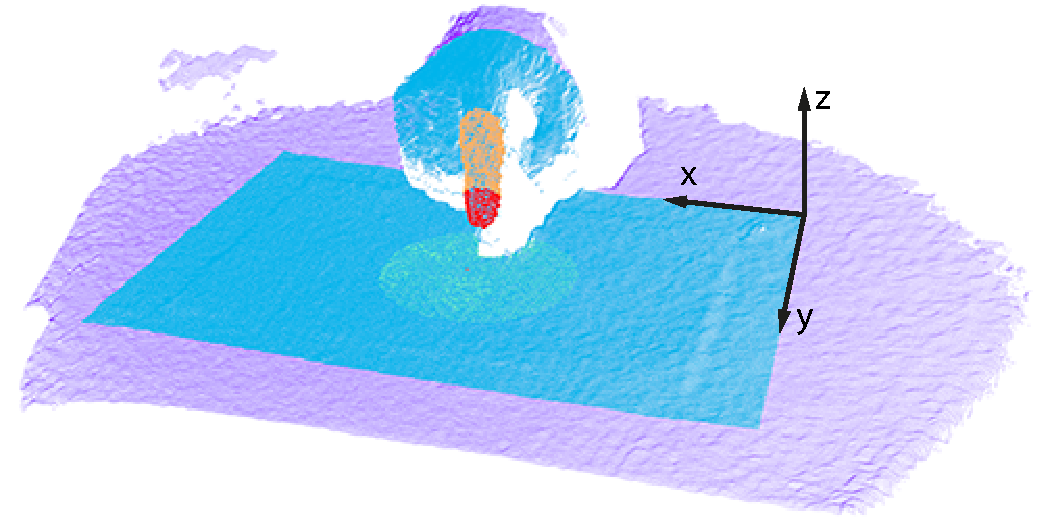
\includegraphics[width=\linewidth]{figures/pointcloud.pdf}
    \caption{Segmented sensor image with points within the interactive surface (blue), the ROI plane (cyan), the detected fingers (yellow) and the user pointer (red).}
    \label{fig:pointcloud}
\end{figure}

\begin{figure}
    \centering
    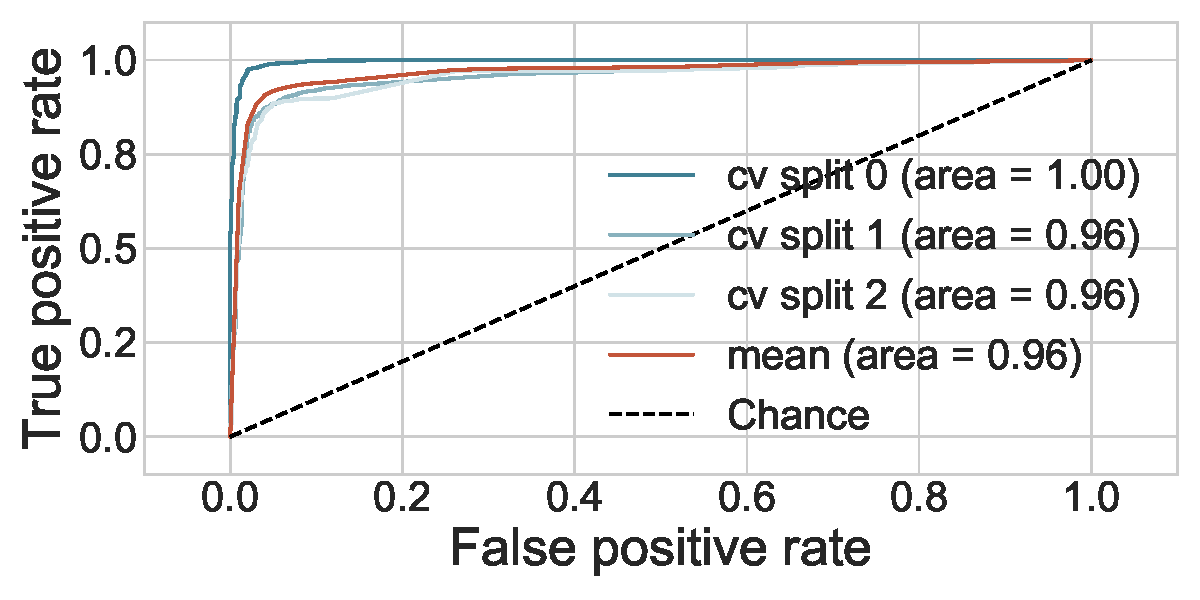
\includegraphics[width=\linewidth]{figures/roc_auc.pdf}
    \caption{Performance of the fingertip touch classification with 3-fold cross validation. Each split trains on two finger types (among three) and validates against the remaining one.}~\label{fig:roc_auc}
\end{figure}
}

We recruited 12 participants, all right handed, without requirement on gesture typing experience.
A repeated measures within-subjects design was used. There were 3 conditions (\cdt{device}, \cdt{size} and \cdt{orientation}) and 5 level combinations were evaluated, see \autoref{tab:cdt} below for details. We adopted a 3-symbols naming convention: the first letter represents the DEVICE, the second marks the ORIENTATION and the number represents the scaling factor as SIZE.

The apparatus, see \autoref{fig:system_insitu_0}, implements the system description above. An Intel Realsense camera is used, and the processing is performed on a desktop computer. An Android tablet running custom software produces the audiovisual feedback. The pointer tracked by the system is defined as the point cloud closest to the camera in the depth direction ($y$ on ~\autoref{fig:pointcloud}); there is no explicit finger or hand modeling performed. Instead, the assumption is that the interacting finger is the furthest protruding object from the user.

The task was to write 20 words per level (words taken at random from the most common english words with length between 2 and 5 letters) with maximum 7 attempt to complete 5 correct input for each word. The design of the task is similar to \cite{Quinn2016} and allows novice users to focus on the physical execution instead of the shape recollection, effectively emulating a proficient bahavior even for novice users. After each level, participants were offered to take a break before moving to the next one. Finally, participants were asked for their feedback using the NASA Task Load Index~\cite{Hart1988} (NASA-TLX) to assess the perceived workload of completed level.

The experimental design was thus: 12 participants $\times$ 5 \cdt{level} $\times$ 20 \cdt{word} = 1200 trials. For each trial, we had 5 to 7 attemps depending on the error rate, which means a total of 6,000 to 8,400 total samples. After the experiment, we actually recorded 6963 samples.

\begin{table}
  \centering
  \begin{tabular}{l l | r r r r r}
    \smit{LEVEL} & \smit{DEVICE} & \smit{width} & \smit{height} & \smit{area}& \smit{ratio} & \smit{$CD_{gain}$} \\
    % \midrule
    \hline
    \cdt{OP1} & \cdt{optical} & 9.4 & 4.7 & 44.2 & 2 & 1 \\
    \cdt{OP2} & \cdt{optical} & 18.8 & 9.4 & 176.7 & 2 & 1/2 \\
    \cdt{OL2} & \cdt{optical} & 25.6 & 6.9 & 176.6 & 3.7 & 1/1.7 \\
    \cdt{OP4} & \cdt{optical} & 37.7 & 18.9 & 712.5 & 2 & 1/4 \\
    % \midrule
    \hline
    \cdt{tp1} & \cdt{tablet} & 9.4 & 4.7 & 44.2 & 2 & 1 \\
  \end{tabular}
  \caption{Design of the experiment. Level name, device type, dimensions (in $cm$), area (in $cm^2$), ratio and control/display gain for all 5 combinations used in the experiment.}~\label{tab:cdt}
\end{table}

% =============================================================================
\section{Results}
% =============================================================================
The dependent variables we analyse are the success rate, the time taken per trial and the trace data when available. From these, we computed the dependent measure error rate defined as the percentage of unsucessful attempts as well as the text entry rate measured in Words Per Minute (WPM), as in~\cite{Markussen2014}, according to the following formula\footnote{$WPM = |T|/s \times 60/5$ where $|T|$ is the length of the transcribed string, s is time in seconds}.

We found one input word (\cdt{lay}) presented some very unusual behavior. Its error rate was at $89.5\%$ while the \cdt{WORD} mean was $20.1\%$ and no other word had an error rate higher than $30\%$. The reason was that the recogniser promoted words of higher prior probability in the language model, \textit{``Larry''}, \textit{``last''} or \textit{``Katy''}. For the all subsequent analysis of error rate, \cdt{lay} was removed from the dataset.

\subsection{Effect on error rate}
A statistical analysis showed a significant main effect of DEVICE ($F_{1,11} = 37.77, p < 0.0001$) on error rate with mean value for \cdt{TP1} and \cdt{OP1} equal to 6.2\% and 26.1\%, respectively, see \autoref{fig:err_DEVICE_SHAPE}. A statistical analysis also showed a significant main effect of \cdt{SIZE} ($F_{2,22} = 10.99, p < 0.001$) on the error rate. Finally, an ANOVA on \cdt{TP1}, \cdt{OP2}, \cdt{OP4} and \cdt{OL2} did not show a significant main effect ($p = 0.11$) even though \cdt{OPTICAL} is on average higher than \cdt{TABLET}. In other words, among all levels of the experiment, only \cdt{OP1} shows a significant higher error rate.

\marginpar{
\begin{figure}
    \centering
    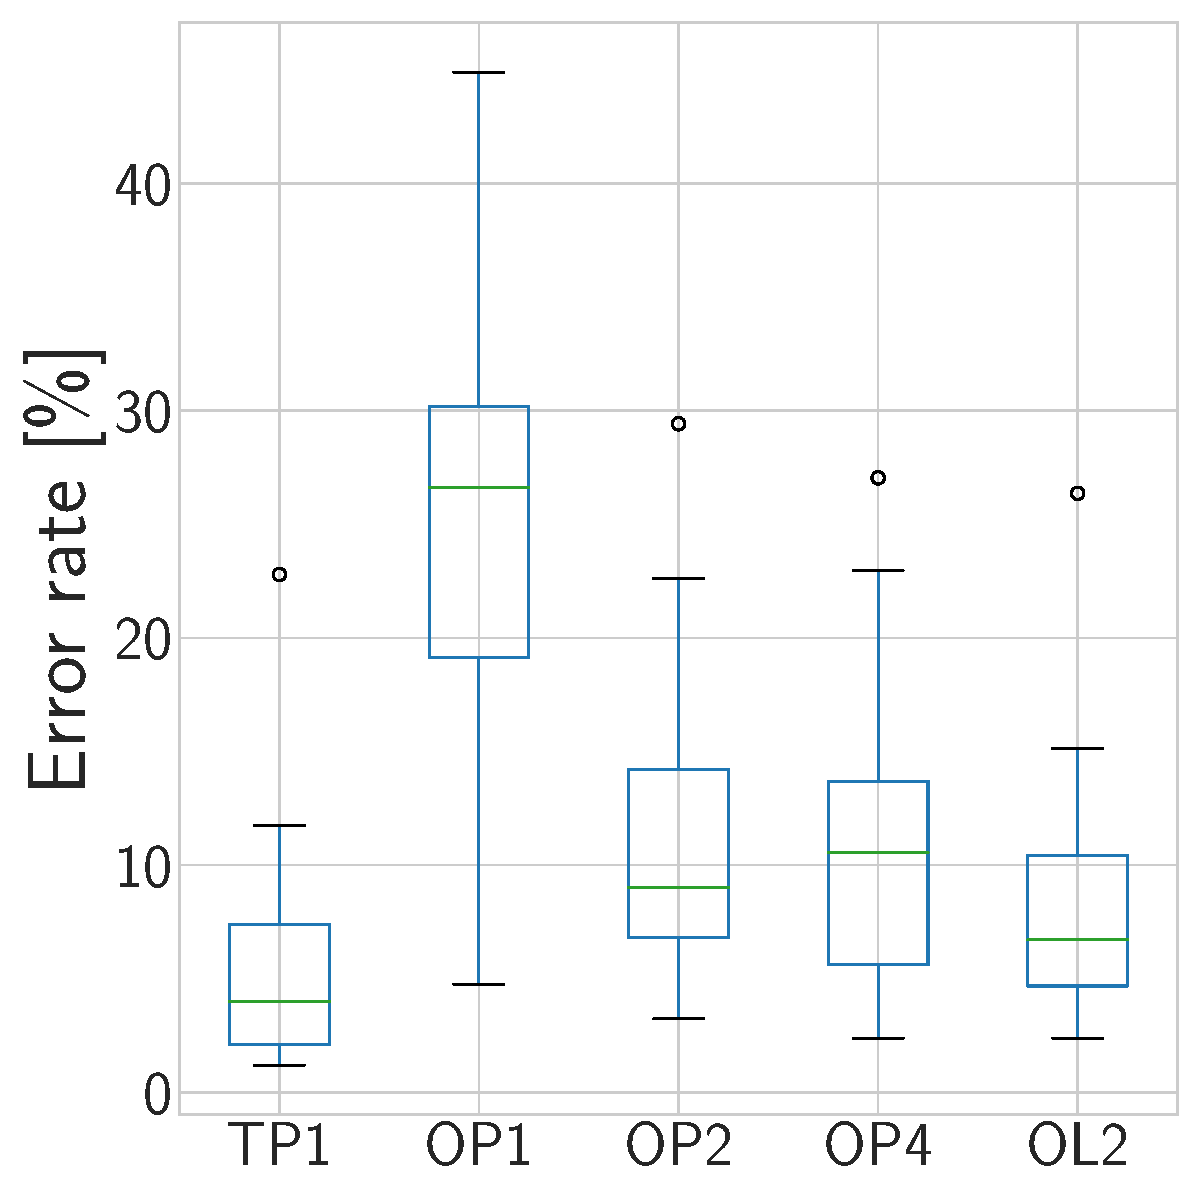
\includegraphics[width=\linewidth]{figures/err_DEVICE_SHAPE.pdf}
    \caption{Effect of levels on error rate.}
    \label{fig:err_DEVICE_SHAPE}
\end{figure}

\begin{figure}
    \centering
    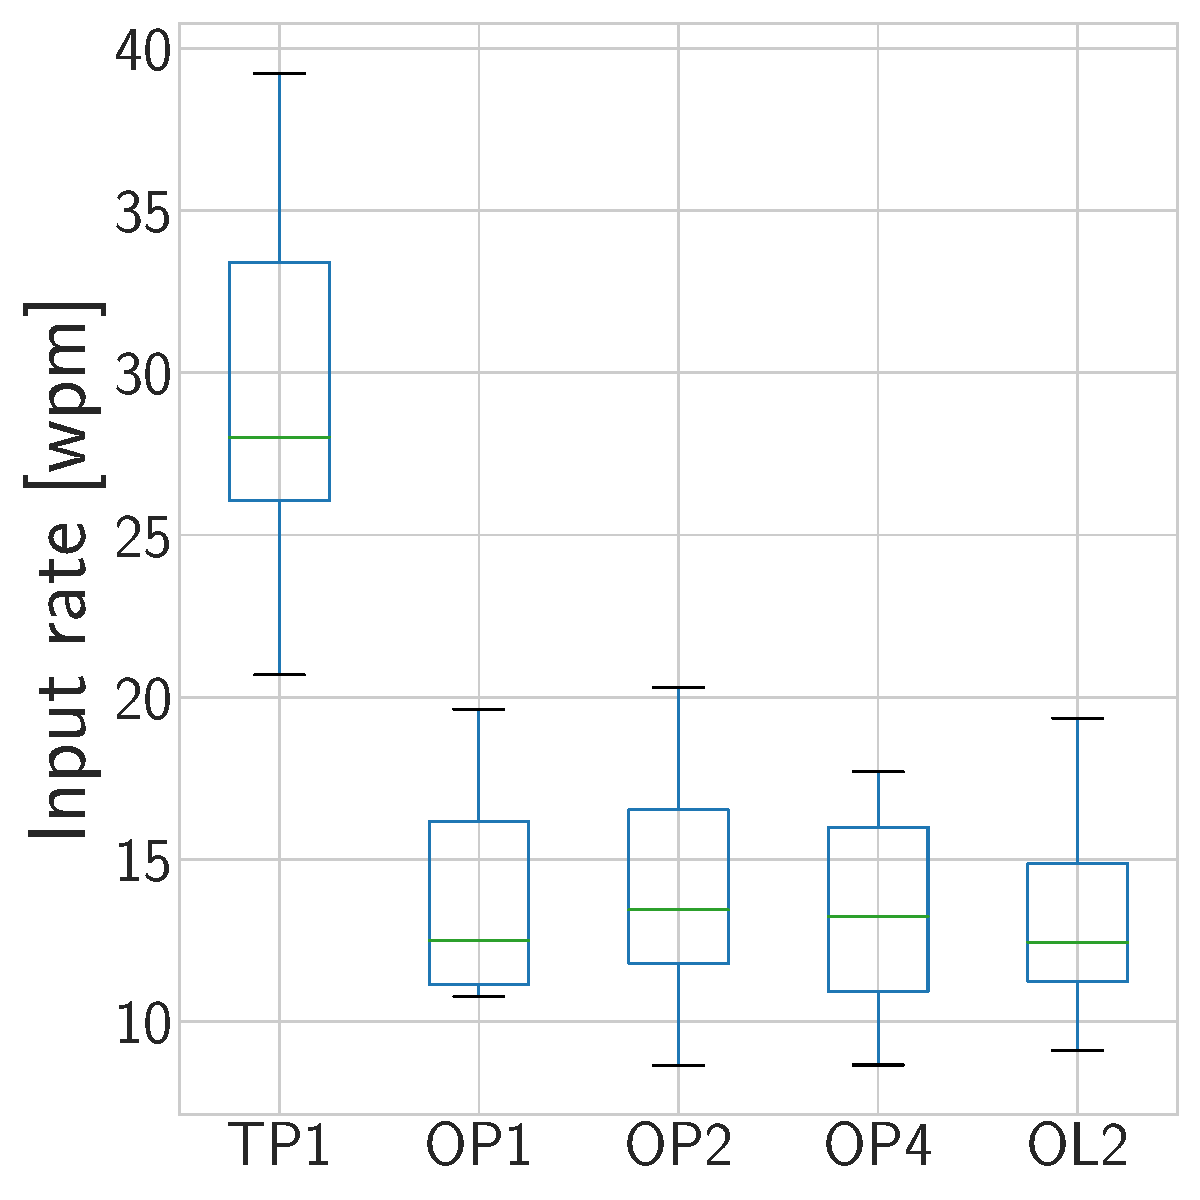
\includegraphics[width=\linewidth]{figures/wpm_DEVICE_SHAPE.pdf}
    \caption{Effect of levels on input rate.}
    \label{fig:wpm_DEVICE_SHAPE}
\end{figure}
}

\subsection{Effect on input rate}
A statistical analysis showed a significant main effect of \cdt{DEVICE} ($F_{1,11} = 90.15, p < 0.0001$) on input rate, see \autoref{fig:wpm_DEVICE_SHAPE}, with mean values for \cdt{TP1} and \cdt{OP1} equal to $29.2 WPM$ and $13.7 WPM$, respectively. We also looked at pairwise comparison\footnote{Post-hoc analysis were adjusted using Bonferroni correction.} for \cdt{OPTICAL} and could not find a statistical difference in the mean input rate. The input rate achieved by the participants in \cdt{TP1} is in-line with what can be expected from novice users after the time of the experiments~\cite{Kristensson2004}. The averaged 54\% lower input rate in \cdt{OPTICAL} should be compared with other similar results, as~\cite{Markussen2014} with 57\% after 10 sessions, that compare direct and indirect input modality for mid-air gesture typing.

\subsection{Effect of orientation}
The design of the experiment also includes \cdt{ORIENTATION}. This condition has so far been excluded from the SIZE analysis and can be difficult to apprehend since not only the \cdt{ORIENTATION} of the visual feedback changes, but its size also. The main result is the average pointer speed in display space at $303.75 pixel/s$, higher than the PORTRAIT orientation at an average $228 pixel/s$. It is important to keep in mind that the keyboard area in LANDSCAPE ($61cm^2$), bigger than PORTRAIT ($44cm^2$), which can explain the faster pointer speed but is not responsible for a higher input rate due to longer traces to produces.

\subsection{Qualitative data}
At the end of the experiment, participants were invited to provide some informal feedback, rank the different level in order of preference and fill in the NASA-TLX form, the tablet interaction was ranked best by all participants except one. \cdt{OP4} was consistently ranked last, while \cdt{OP2} and \cdt{OL2} had equal ranking in second position. The NASA-TLX data shows that participants describe \cdt{OP4} as the most physically demanding interaction. Participants graded \cdt{OP1} and \cdt{OP4} 20\% higher than \cdt{OP2} and \cdt{OL2} on the scale of effort and frustration. Finally, \cdt{OP1} was graded as having lowest level of performance and highest mental and temporal demand.

\section{Discussion}

% We proposed a machine learning approach to fingertip touch detection. This problem is traditionally addressed by hand-tuning parameters and thresholding. In contrast, we showed that using a machine learning approach can solve the problem and generalise well enough to be used in an experiment with 12 unseen participants. One improvement could be to delegate the feature extraction step (an histogram of z-values in our case) to a model capable of inferring features directly, such as a convolutional neural network. Since the data is cheap to record, we could see this approach being used for many specific cases.

We conducted a user study investigating the usability of the system and showed that for control dimension at least twice the display dimension novice users were capable the same error rate at half the input rate. We also showed that at the same $CD_{gain}$, the error rates were dramatically higher. Also, the experiment showed a constant input rate across display sizes and aspect ratios. Accot et al.~\cite{Accot2001} showed that task with high index of difficulty would exhibits a u-shaped curved with size. Since we did not observe such a behavior, this puts in question whether gesture typing for novice users is “hard enough”.

The constant input rate however shows that participants are capable of adapting their motor speed across all investigated scales. Participants also varied the display pointer speed, especially in \cdt{OL2} when presented with a bigger display surface. Because participants are capable of adapting their motor behavior and their control bahavior, another explanation for the upper bound in text input is that the indirect nature of the interaction is the limiting factor.

Participants feedback showed that \cdt{OP1} was a demanding interaction, and that increasing the surface size to the extent of \cdt{OP4} was also physically demanding. We would therefore recommend sizes \cdt{OP2} or \cdt{OL2} for interaction, noting that the performance is also dependent on the $CD_{gain}$). Some participants reported the texture having an impact of the interaction. Levesque et al.~\cite{Levesque2011} have used friction in a dynamic manner to improve target acquisition. Given the relatively low performance of the participants, it could be interesting to explore if tactile feedback could help controlling an indirect pointer.

% =============================================================================
\section{Conclusion}
% =============================================================================
We developed a system that affords gesture typing on arbitrary flat surfaces using depth camera tracking, and demonstrated a machine learning approach to the issue of detecting touch for fingertips which is effective for this mode of control. We designed an experiment with two research goals in mind. First, we compared the typing performance of our optical indirect system against a control condition which was a direct interaction on a tablet. Second, we studied the influence of size and aspect ratio of the input surface on gesture typing performance. We showed that the participants could enter text at half the input rate and the same error rate on surface at least twice the size of the visual feedback. We also showed that the input rate is largely independent of surface size across the range of sizes we were able to examine. Gesture typing has promise for interaction outside of mobile devices, e.g. for motor impaired users who struggle with capacitive touch technologies. This paper indicates that while camera-tracked gesture typing performance is usable, input rates are lower than touchscreen performance, and this is not influenced by scaling of the input.

\section{Acknowledgements}
We thank the European Commission and Horizon 2020 for funding this research (award number 643955).

\balance
\bibliographystyle{acm-sigchi}
\bibliography{collection}

\end{document}